\section{Entities}\label{sec:01}
In order to access the Bakery System, You should be registered as a User therein. 
After the registration a User can log in to the system using their username and password.

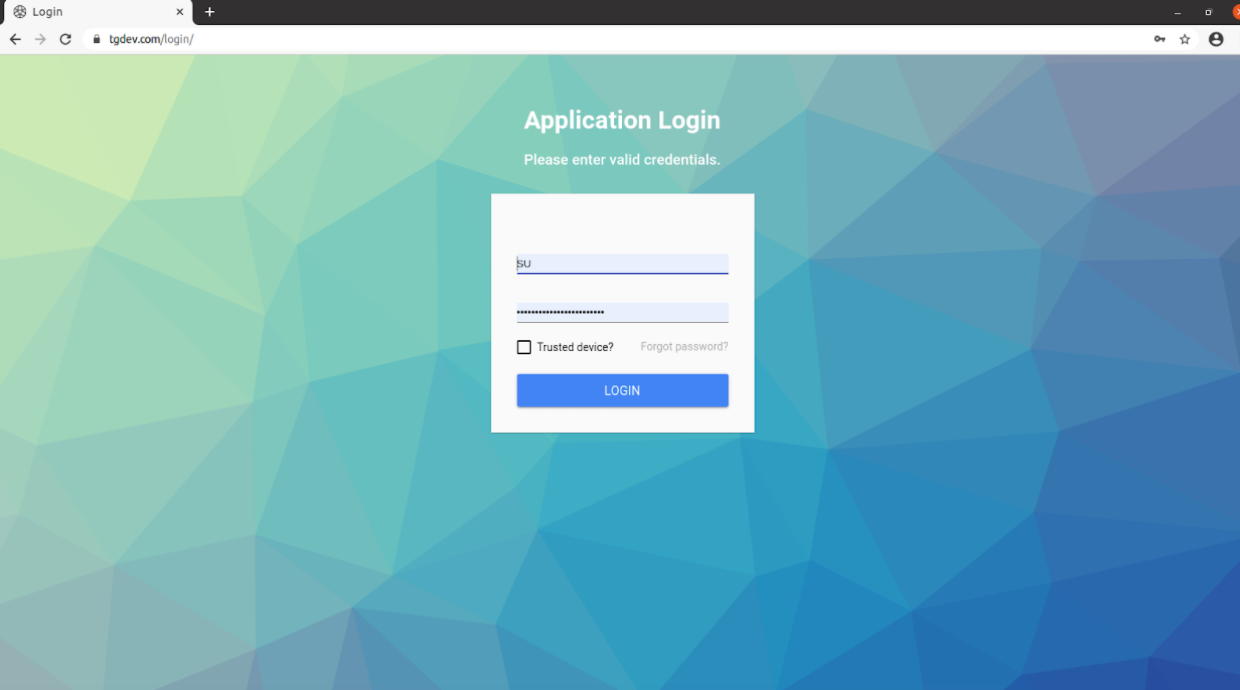
\includegraphics[width=\textwidth]{sections/01-chapter/images/login.png}

The System consists of multiple entities - key players in the system, which are used.

You can review them by clicking on :

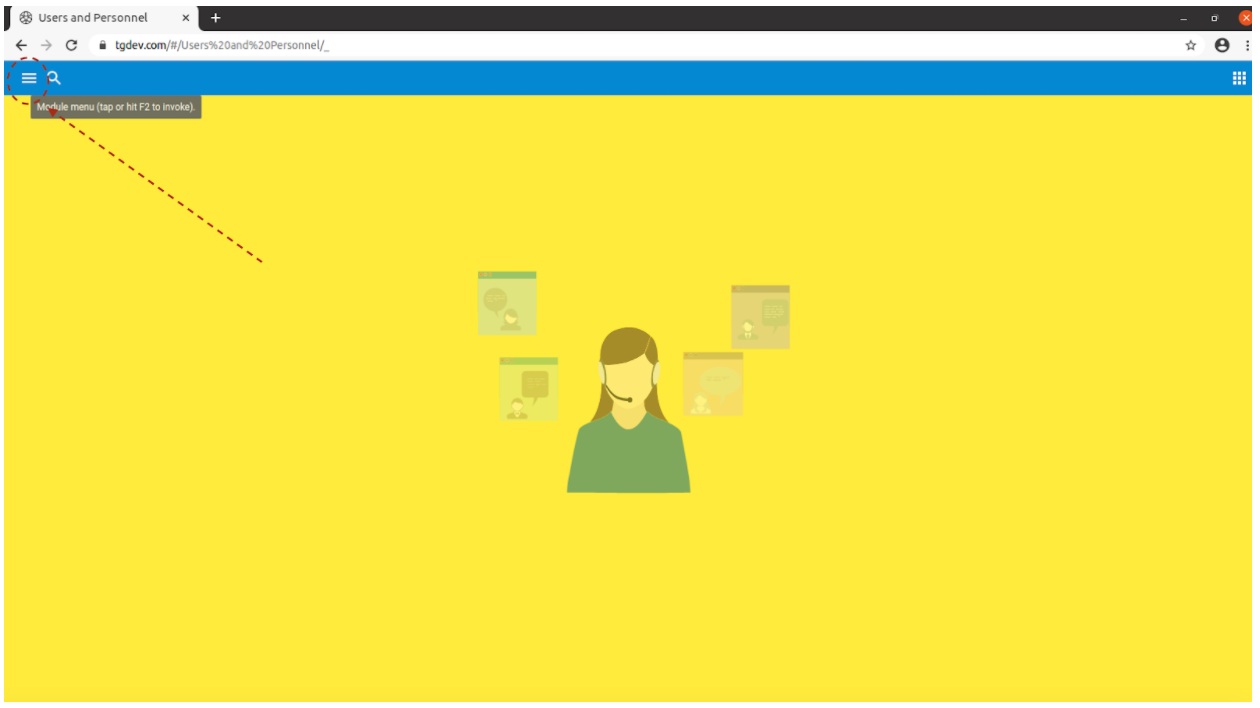
\includegraphics[width=\textwidth]{sections/01-chapter/images/review1.png}
% \includegraphics[height=5cm]{review2.png}\\

Depending on the role a user has in the system, they can either have the ability to register and edit some entities or not. 
The key entities are:

- Person 

- Manager

- Carrier

- Location

- Order

- Product

- Employment

- OrderItem

\subsection{Person}
A person represents an entity that is any person (they can be either one of the workers in a bakery or just a person).

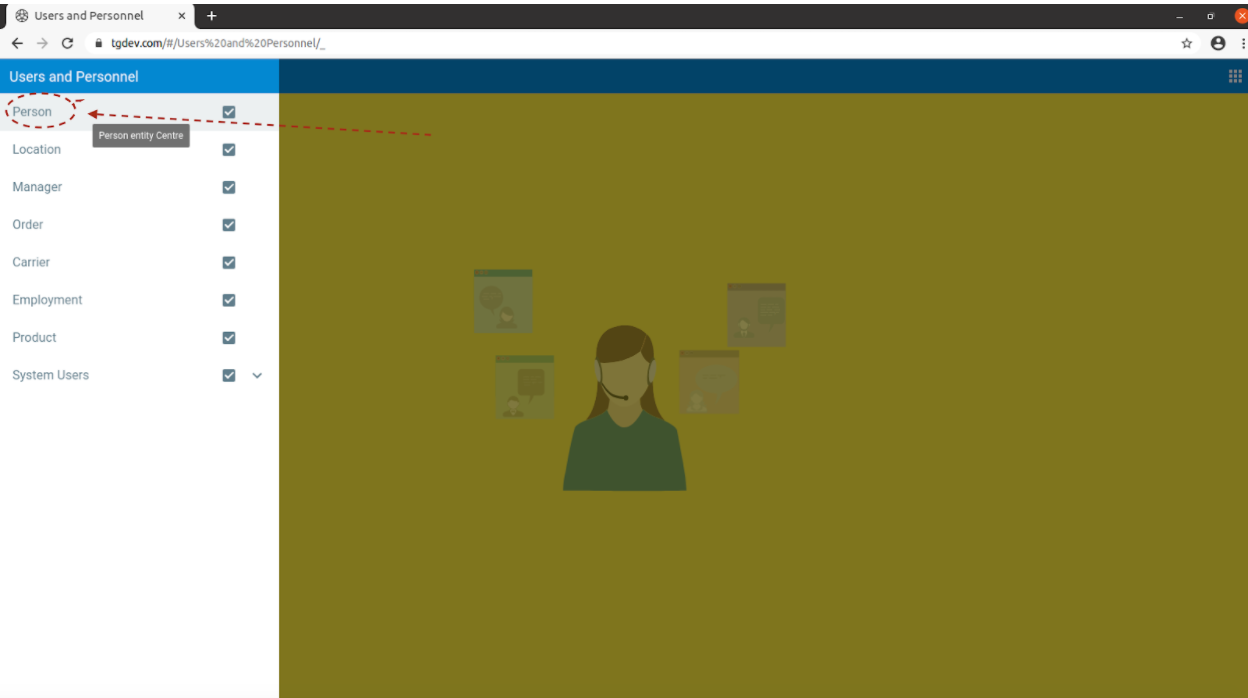
\includegraphics[width=\textwidth]{sections/01-chapter/images/person1.png}

\textbf{Creation of a new Person}

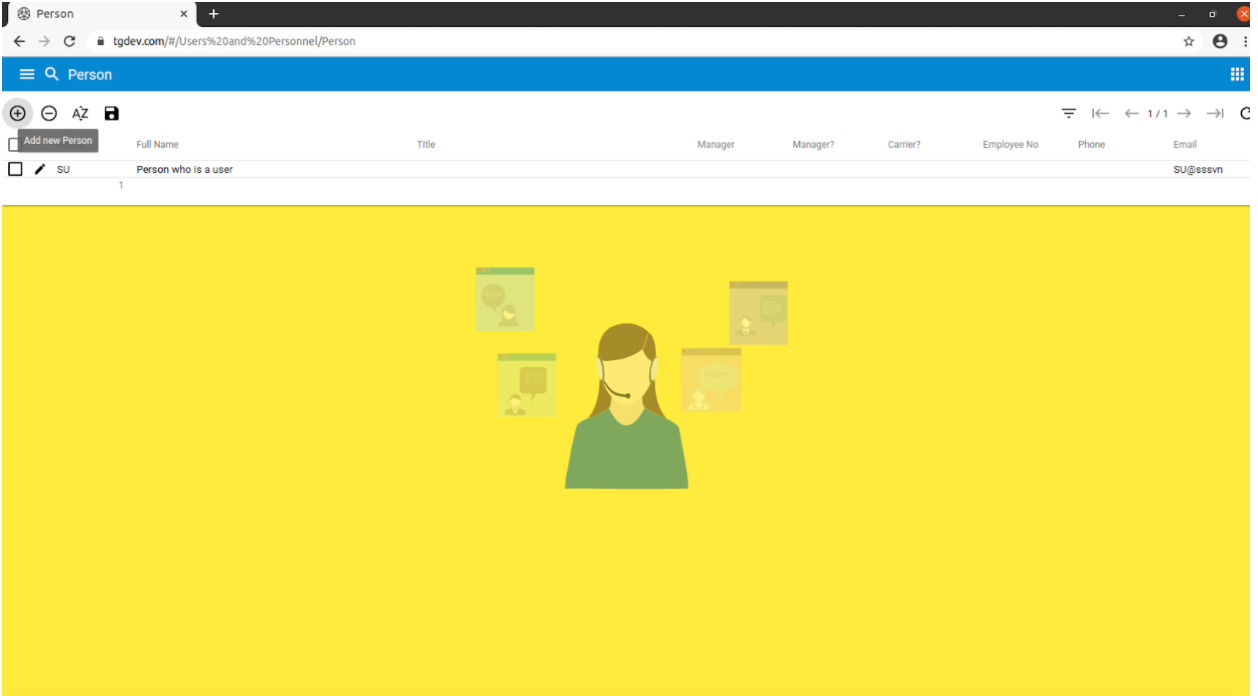
\includegraphics[width=\textwidth]{sections/01-chapter/images/person2.png}

To create a new person you need to  fill in the important fields such as:

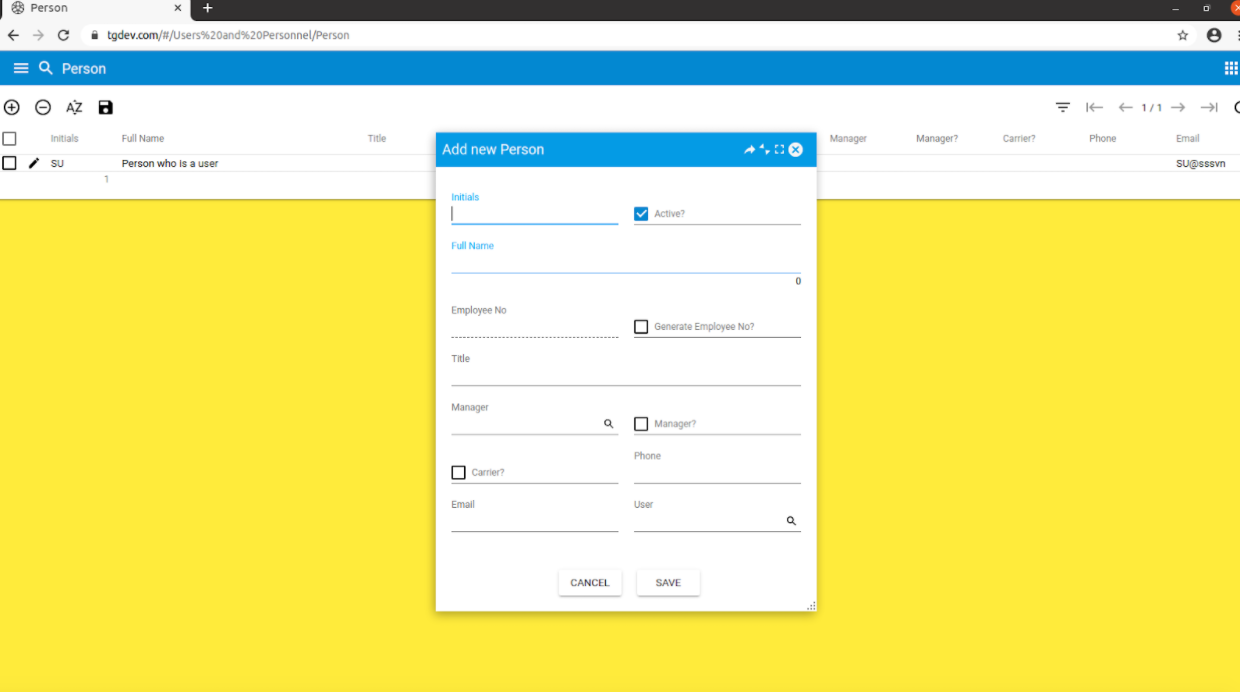
\includegraphics[width=\textwidth]{sections/01-chapter/images/person3.png}

- Initials →  required, string, spaces are not allowed in the initials

- Active → required, the indicator of an active participant in the system. The environment cannot interact with inactive Person.

- Title →  optional, person’s position.

- Employee Number → optional, the indicator number of the employee, can be generated automatically, if specified in the checkbox to the right, then position must be specified (cannot be left empty) as well. 

- Phone number → optional String, phone number of a Person

- Email →  optional, String, email

- aManager →  optional, Manager of this employee, this field is required if Employee Number is specified. In other words, every Person who has an employee number must also have a manager.

- Manager? →  optional checkbox, indicates whether this employee is in the manager role

- Carrier? → optional checkbox, indicator of whether this Person is a carrier

- User → optional, a system user associated with this Person

You can search for a Person using the following properties: 

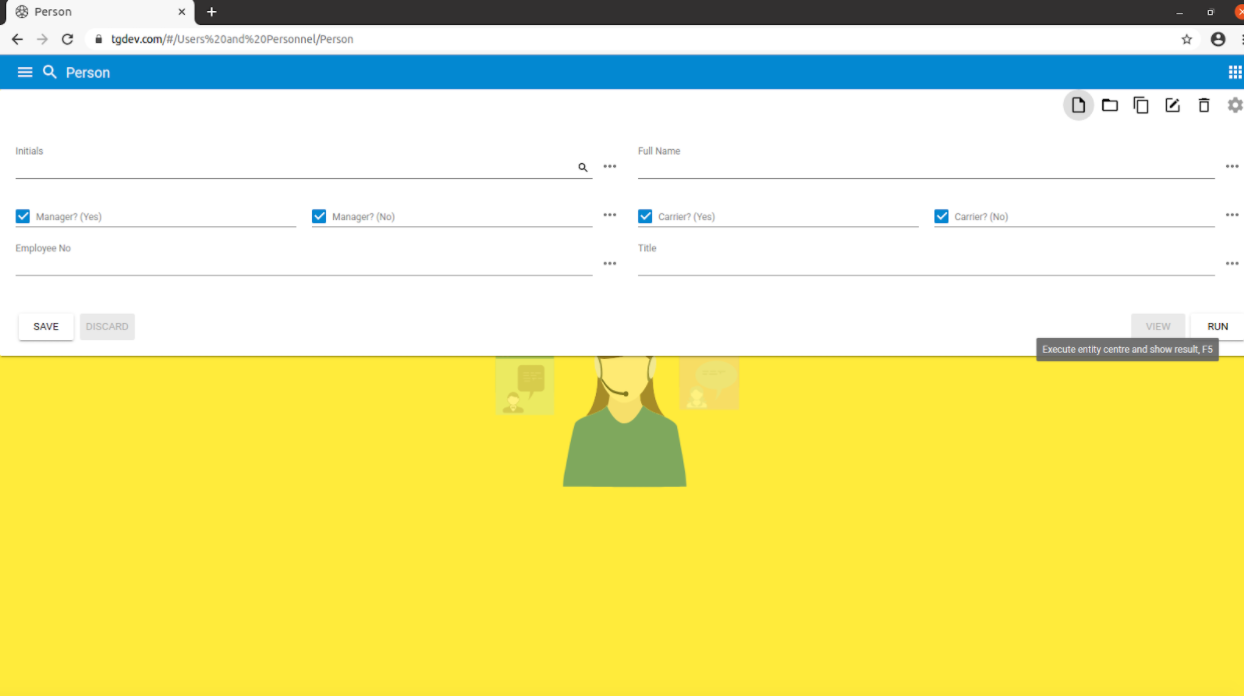
\includegraphics[width=\textwidth]{sections/01-chapter/images/person4.png}

\subsection{Manager}
A manager represents an entity that is technically a person assigned to the manager`s role.

\textbf{Creation of a new Manager}

One cannot add a Manager to the database straightforwardly. 
A manager can be added only during registration of a Person by clicking on Manager? checkbox which indicates that a person is in the manager role now.
An important thing here: Employee number must be specified in order to assign person as a Manager.

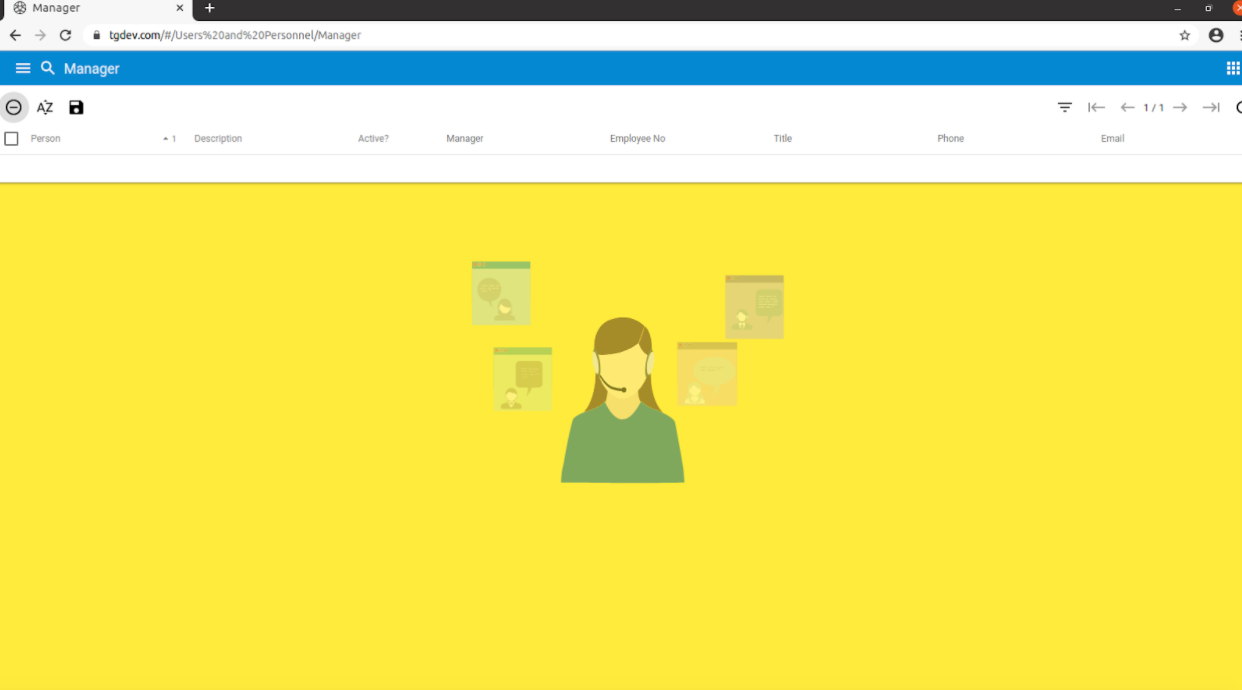
\includegraphics[width=\textwidth]{sections/01-chapter/images/manager1.png}

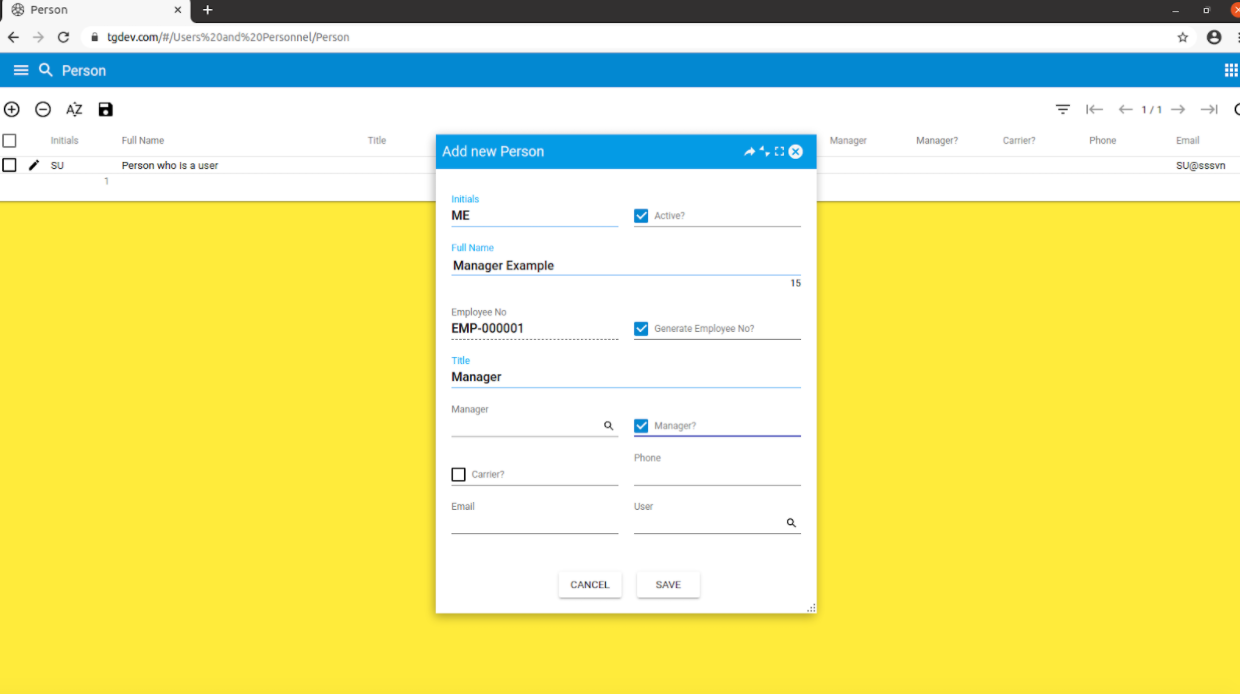
\includegraphics[width=\textwidth]{sections/01-chapter/images/manager2.png}


The required fields for a manager are:

- Employee No → the indicator number of the employee, can be generated automatically, if specified in the checkbox to the right.

- Title → the role, position of an Employee in the Bakery system

In addition, the standard fields are required:

- Initials

- Active? checkbox - which indicates whether the system can further use can interact with the Manager/ The indicator of an active participant in the system. The environment cannot interact with inactive Person.

- Full Name

The rest of the fields are optional and the same as described in Person.

Some of the constraints in this part: Manager cannot manage themselves and Manager cannot manage a non-employee.

\subsection{Employment}

Employment module represents a concept of employment in the bakery and stores all the important information about this process.

In order to look for existing employment, one should choose Employment entity.

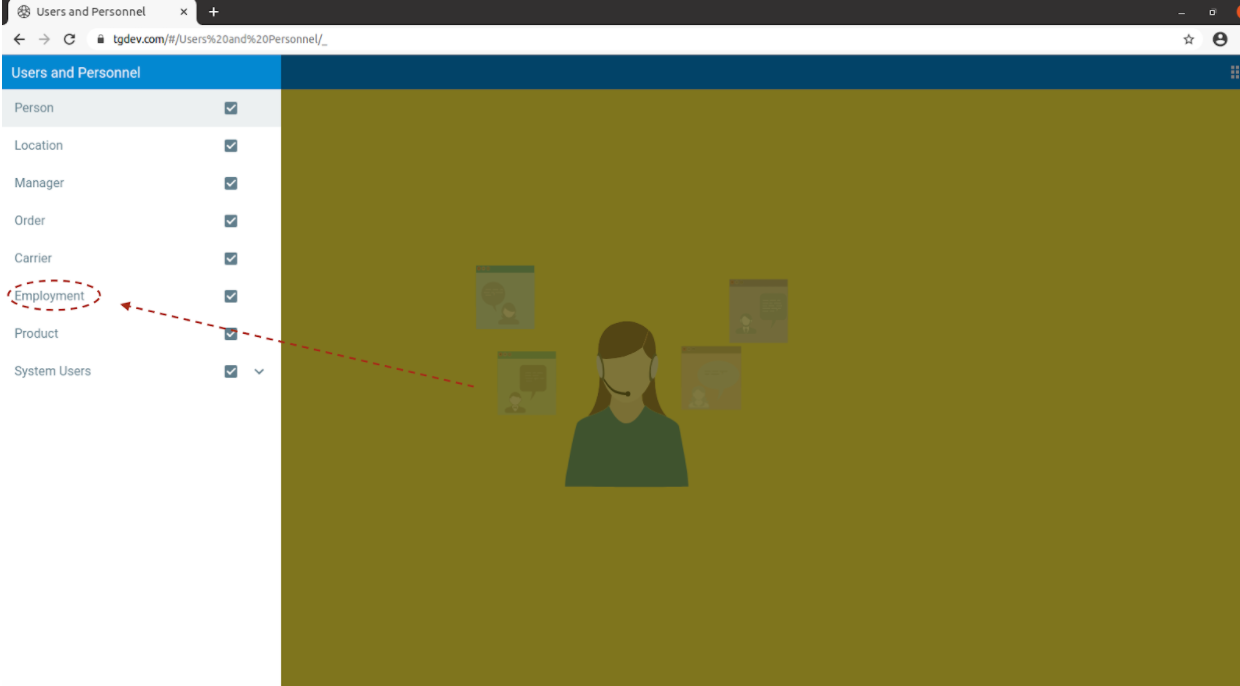
\includegraphics[width=\textwidth]{sections/01-chapter/images/employment1.png}

An employment entity can be found using the following properties:

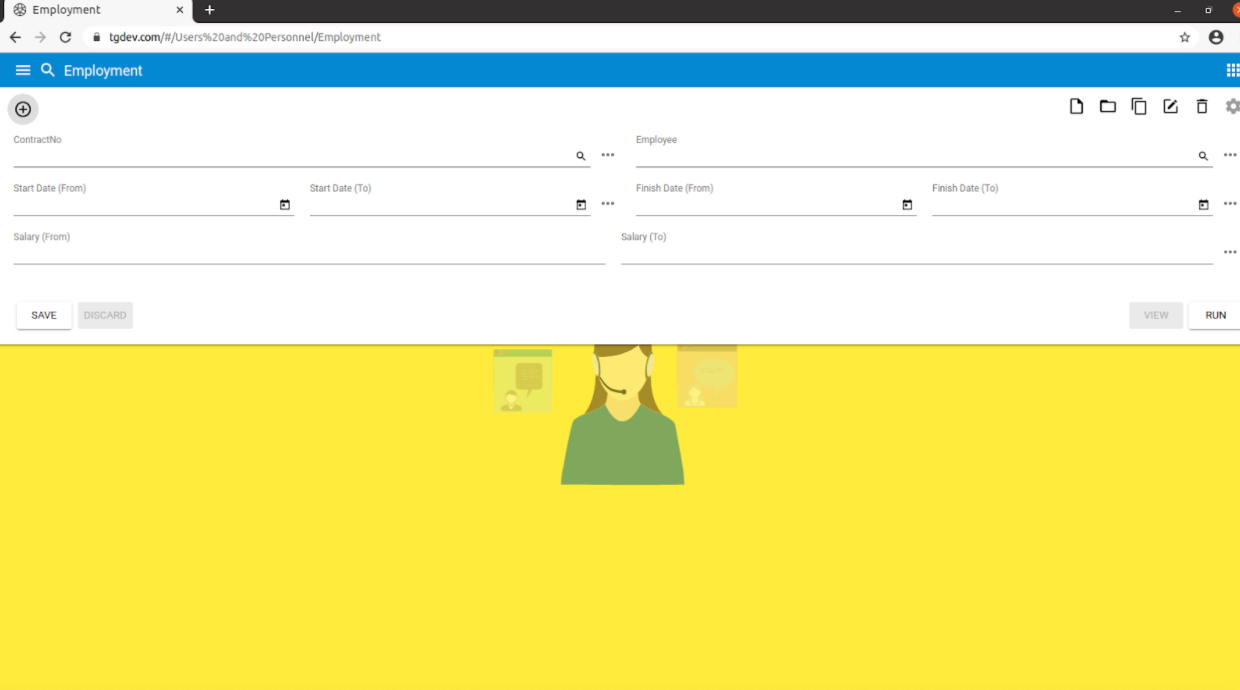
\includegraphics[width=\textwidth]{sections/01-chapter/images/employment2.png}

- ContractNo → String that represents the number of a Contract

- Employee → the initials of a Person Employed

- StartDate (To and From) → range of the starting date of the contract, in which all of the needed Employees will fall

- FinishDate (From and To) → the range of the Finish Dates where the needed employee contracts will fall

- Salary (To and From) → the range of salaries to search in

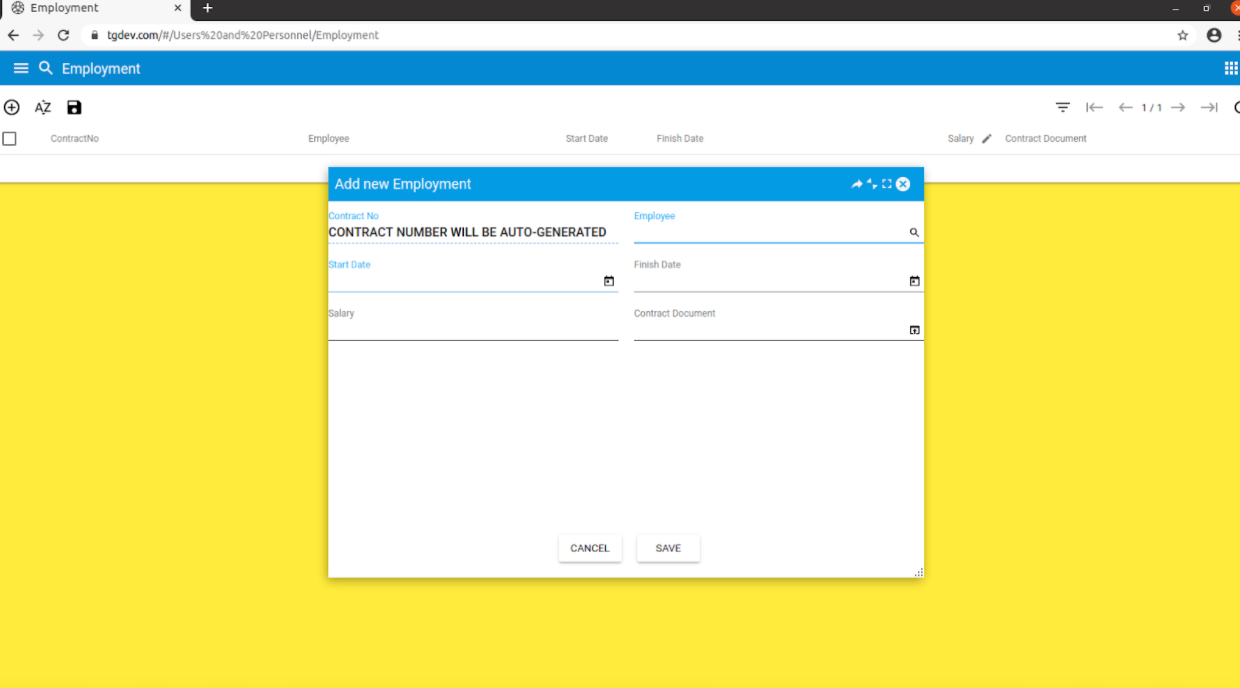
\includegraphics[width=\textwidth]{sections/01-chapter/images/employment3.png}

The registration of new Entity of Employment requires several fields:
- Contract Number - this field is generated automatically for your convenience and is not editable
- Employee - the initials of a person who is employed, required field

- Start Date - start date of the employment, required field

- Finish Date - finish date of the employment, optional field

- Salary - amount which is paid to the employee, optional field

- Contract Document - string that represents the hyperlink to the contract document, optional field

Fields  such as Employee and Start Date are required which means that they cannot be left empty, while Finish Date and Salary may be blank.

The Start and End Dates can be chosen from the popped up calendar icon:

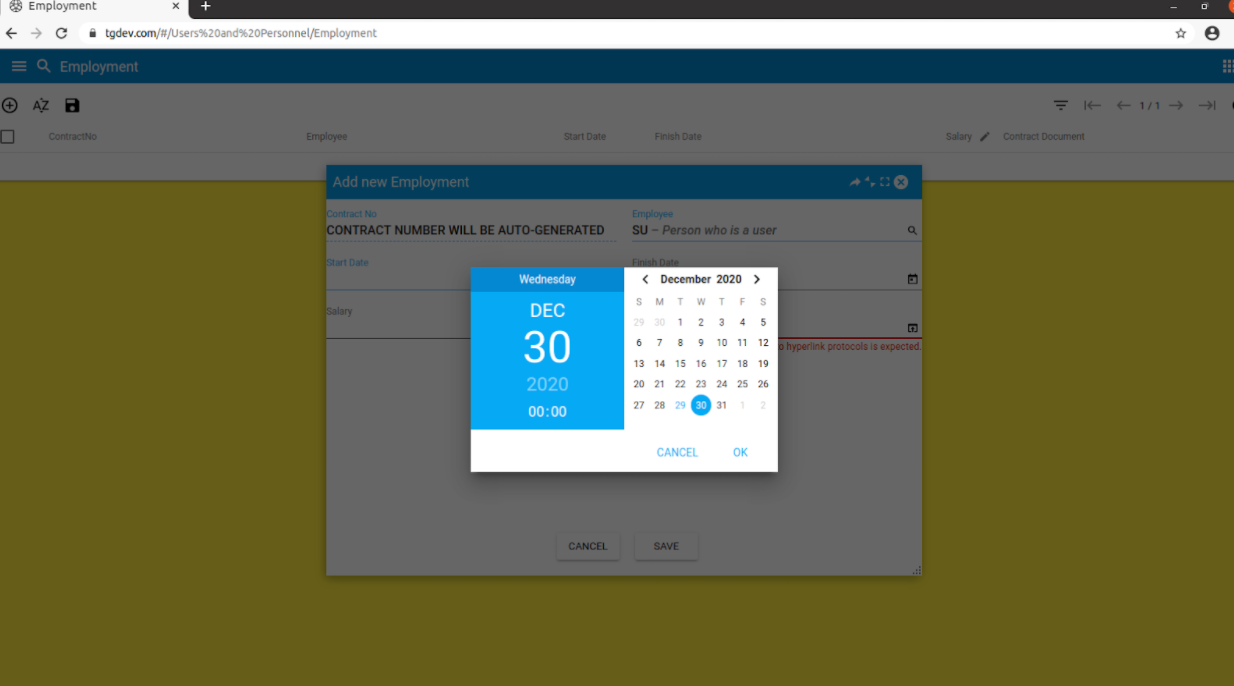
\includegraphics[width=\textwidth]{sections/01-chapter/images/employmentdates.png}

To save the entered information you need to click on the ‘Save’ button. 

To cancel the process and close the form to click on the ‘Cancel' button.

\subsection{Location}

The Location Entity represents a location where a bakery has one of its either distributing or production points. 

One can search through the list of register Location using the following fields:

- Location → the address of the Location

- Description → optional field, the description of the certain Location 

- Country of Location

- City of Location

- Address of Location

- Phone number on a Location

- Range of employee amount

% 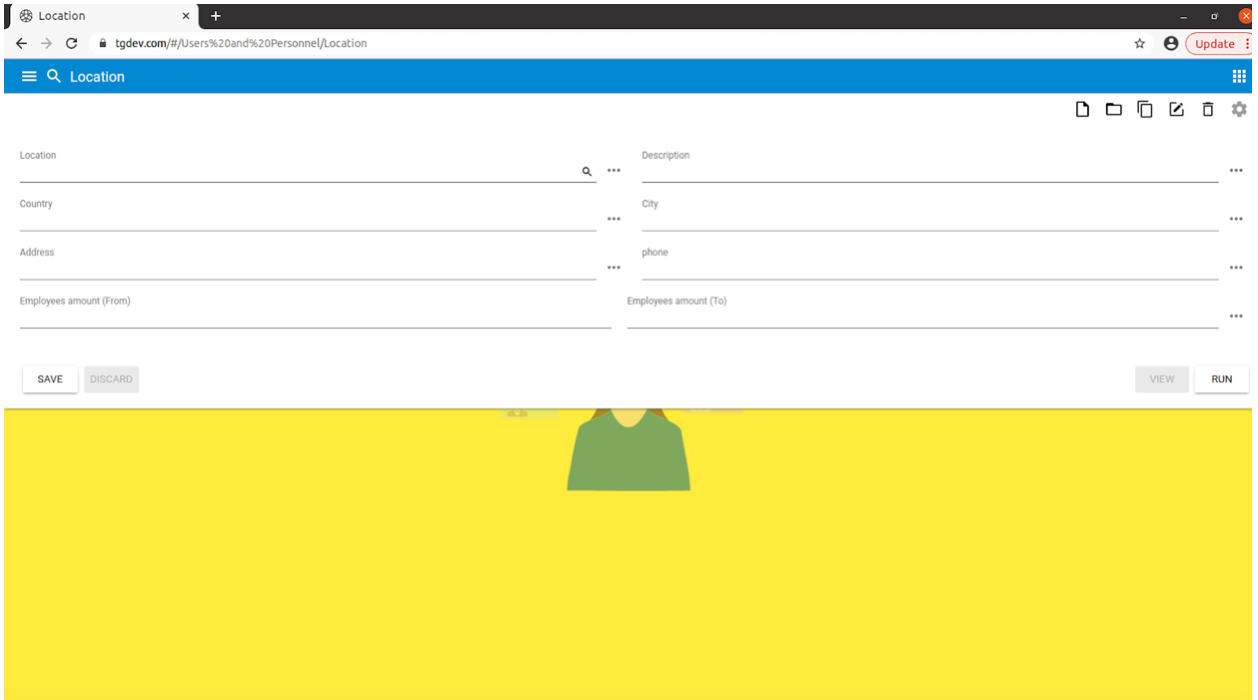
\includegraphics[height=5cm]{location1.png}\\

For the registration of a new Location one should run the search and then press the + sign:

% 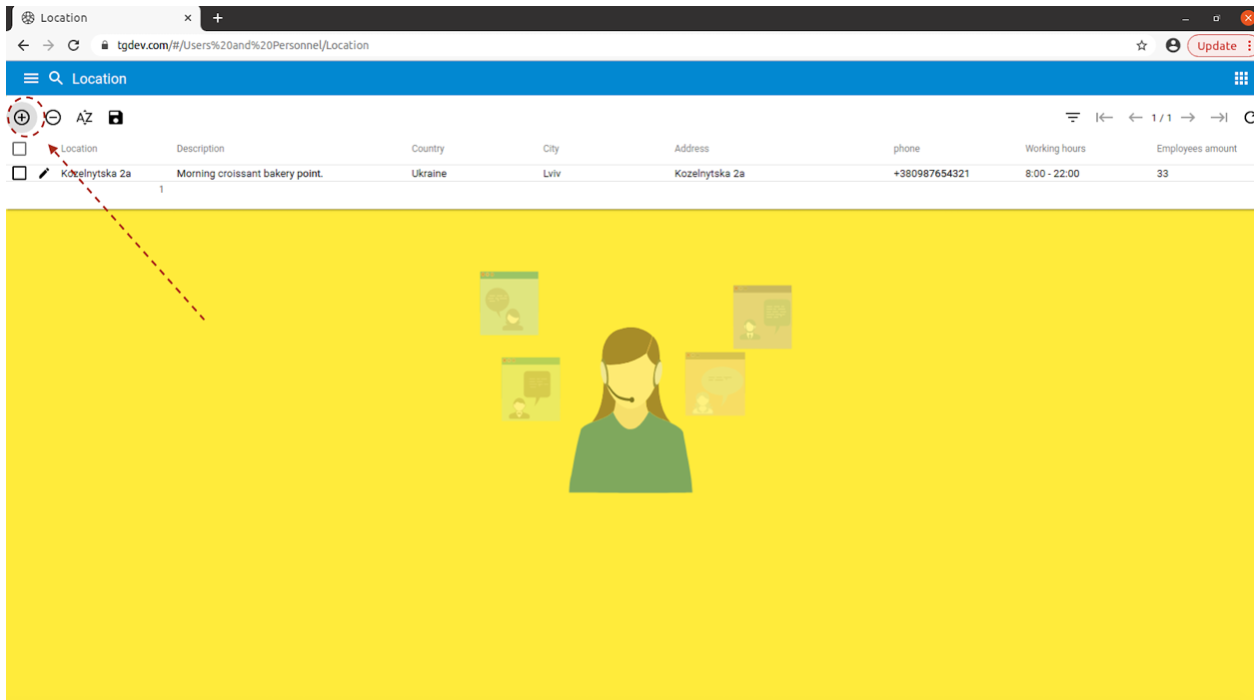
\includegraphics[height=5cm]{location2.png}\\

The Entity depends on a variety of required information. The mandatory fields are highlighted blue and include:

% 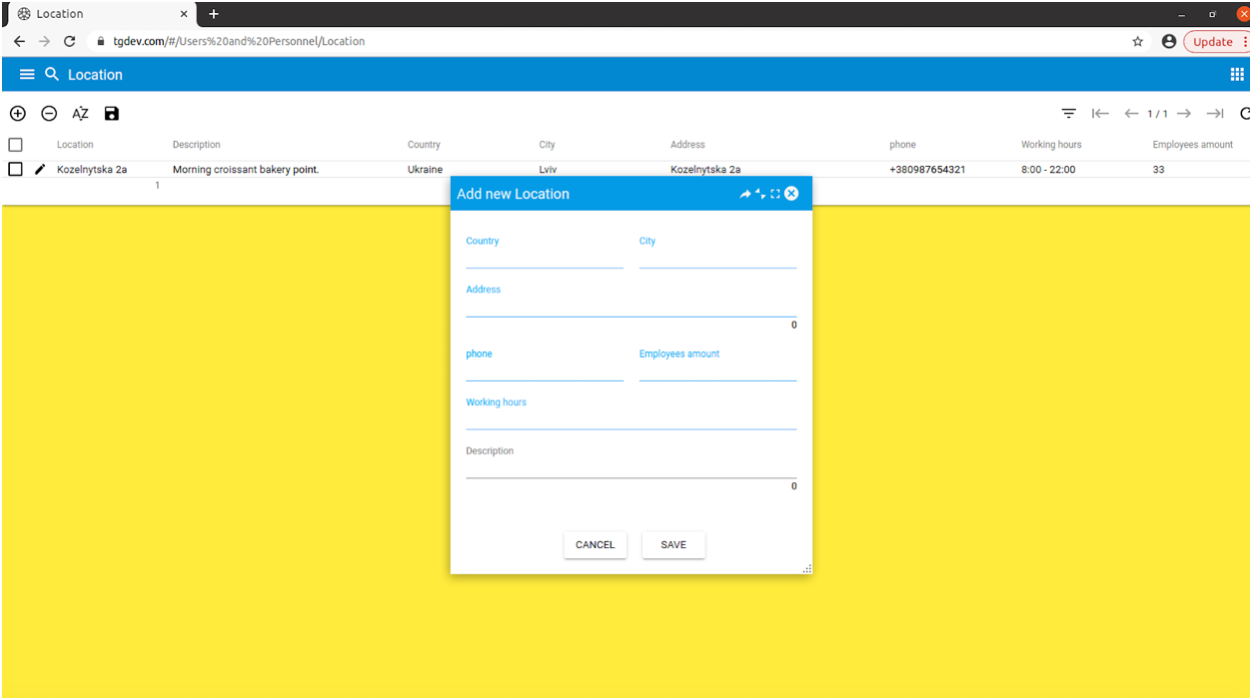
\includegraphics[height=5cm]{location3.png}\\

- Country of the location → Required, String

- City → Required, String

- Address → Required, String that represents street and house number

- Phone → Required, String that represents the phone number of the location, letters are not permitted to be types in this field

- Employees amount → Required, Number that represents number of employees on the location

- Working hours → Required, String that represents the working hours of a location

The additional optional field is the description.

\subsection{Product}

Product represents a good which is produced and sold by the bakery.

To search for a Product one can select the following search criteria:

- Product, which is the name of the product

- Description of the product

- Price range of the products

% 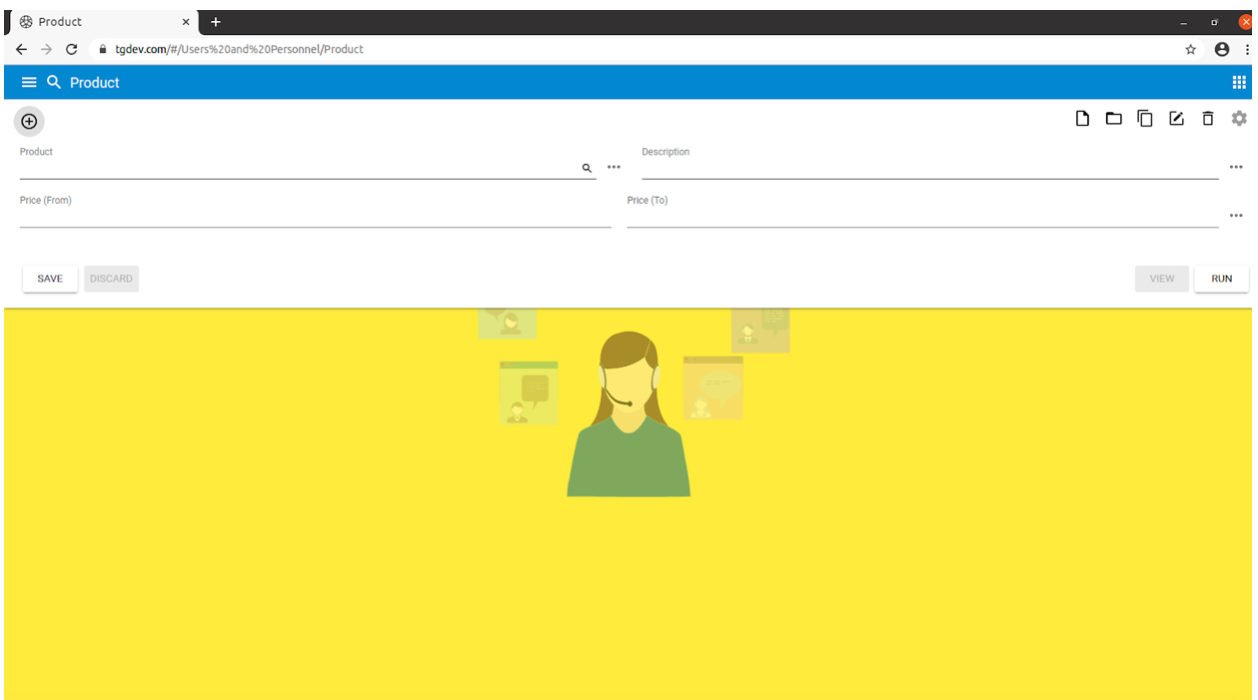
\includegraphics[height=5cm]{product1.png}\\

As a system user aka Manager, to register a new product you need to press the plus button and add the product using the following fields:

- Name → required, String, name of the product, cannot contain any numbers.

- Description → optional, String

- Price → required, Money

- Recipe → Optional, String

% 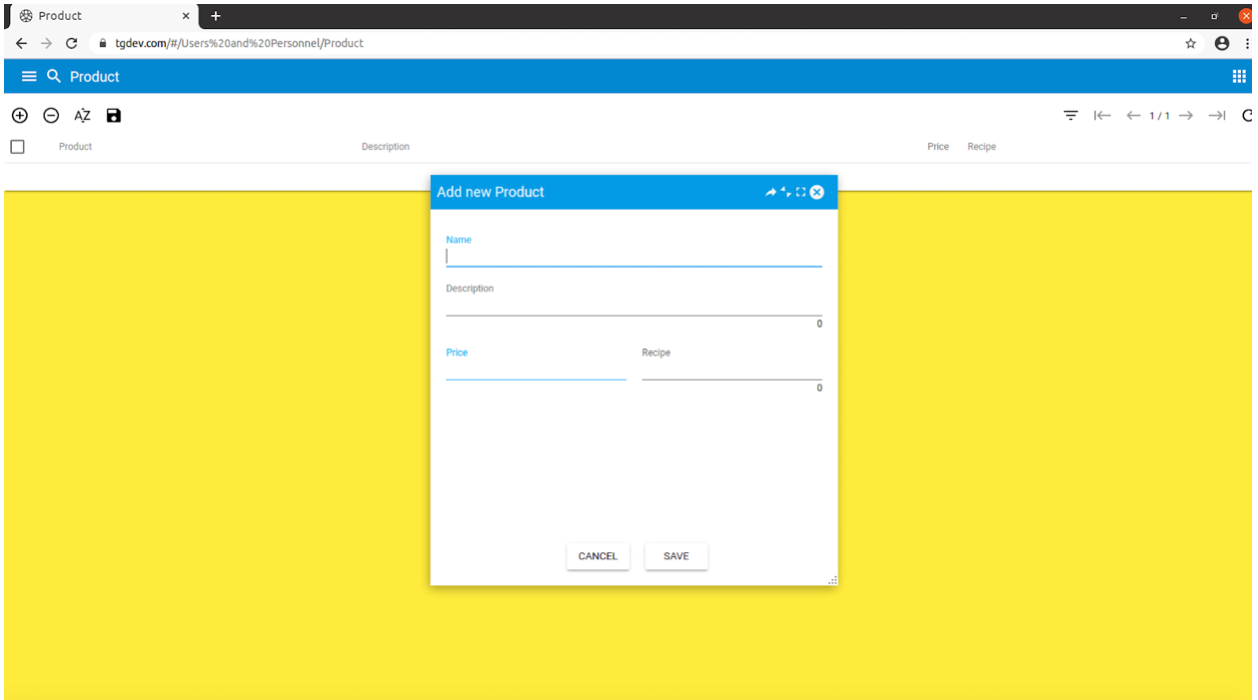
\includegraphics[height=5cm]{product2.png}\\

